\documentclass[11pt, oneside]{exam}
\usepackage{geometry}
\usepackage{pifont}
\usepackage[parfill]{parskip}
\usepackage{tikz}
\usepackage{graphicx}
\usepackage{amssymb}
\usepackage{float}

\geometry{letterpaper}
\usetikzlibrary{arrows,automata}

\newcommand{\cmark}{\ding{51}}
\newcommand{\xmark}{\ding{55}}

\title{CSC416 - Homework 1}
\author{Marshall Bowers}

\begin{document}
\maketitle

\boxedpoints
\pointsinmargin

\begin{questions}

\section*{Regular Languages}

\question
Write English descriptions for the languages generated by the following regular expressions:

\begin{parts}
\part[4] $(0|1|...|9|A|B|C|D|E|F)^+(x|X)$
\newline Any combination of hexadecimal digits (0-9, A-F) one or more times, followed by either an uppercase or a lowercase {\tt x}.
\part[4] $(a|b)^{*}(a|b|\epsilon)$
\newline A lowercase {\tt a} or lowercase {\tt b} zero or more times, followed by either a lowercase {\tt a}, lowercase {\tt b}, or nothing.
\end{parts}

\question
Write regular expressions for each of the following.

\begin{parts}
\part[4] All strings of lowercase letters that begin and end in {\tt a}.
\newline $a[a-z]^{*}a$
\part[4] All strings of digits that contain no leading zeros.
\newline $[1-9][0-9]^{*}$
\part[4] All strings of digits that represent even numbers.
\newline $([1-9][0-9])^{*}(0|2|4|6|8)$
\part[4] Strings over the alphabet \{a,b,c\} with an even number of {\tt a}'s.
\part[4] Strings over the alphabet \{a,b\} that contain an odd number of {\tt a}'s or an odd number of {\tt b}'s (or both).
\newline $a(aa)^{*}|b(bb)^{*}|a(bb^{*})b(aa)^{*}$
\end{parts}

\question
For each of the following regular expressions determine which of the strings {\tt cc}, {\tt ababb}, {\tt bbcab}, and {\tt ccbbab}
matches it:

\begin{parts}
\part[4] \begin{verbatim}(ab)*c|a*b*c*\end{verbatim}
{\tt cc} \cmark
\newline {\tt ababb} \xmark
\newline {\tt bbcab} \xmark
\newline {\tt ccbbab} \xmark
\part[4] \begin{verbatim}(ab|bc*)+\end{verbatim}
{\tt cc} \xmark
\newline {\tt ababb} \cmark
\newline {\tt bbcab} \xmark
\newline {\tt ccbbab} \xmark
\part[4] \begin{verbatim}[ab]*cc?(ab)*\end{verbatim}
{\tt cc} \cmark
\newline {\tt ababb} \xmark
\newline {\tt bbcab} \cmark
\newline {\tt ccbbab} \xmark
\end{parts}

\section*{Lexical Specifications}

\question[3]
Given the string {\tt abbbaacc} and alphabet \{a,b,c\} what tokenization will the following lexical specification produce?
\begin{verbatim}
Token Class      Regex
-----------      -----
     A            b+
     B            ab*
     C            ac*
\end{verbatim}
{\tt <B, abbb>}
\newline {\tt <B, a>} or {\tt <C, a>}
\newline {\tt <B, a>} or {\tt <C, a>}
\newline {\tt <A, bbb>}

\question[3]
Given the string {\tt babac} and alphabet \{a,b,c\} what tokenization will the following lexical specification produce?
\begin{verbatim}
Token Class      Regex
-----------      -----
     A            a(ba)*
     B            b*(ab)*
     C            abc
     D            c+
\end{verbatim}
{\tt <B, bab>}
\newline {\tt <A, a>}
\newline {\tt <D, c>}

\question[6]
Given the following lexical specification and alphabet \{0,1\}, which of the below strings will be successfully tokenized?
\begin{verbatim}
Token Class      Regex
-----------      -----
     A            (11)*
     B            01+
     C            10+
\end{verbatim}
\begin{enumerate}
\item 1000001 \cmark
\item 1110010 \cmark
\item 01100100 \cmark
\item 10011001 \cmark
\end{enumerate}

\section*{Finite Automata}

\question
Explain in informal English what each of these finite-state automata recognizes.

\begin{parts}
\part[5] 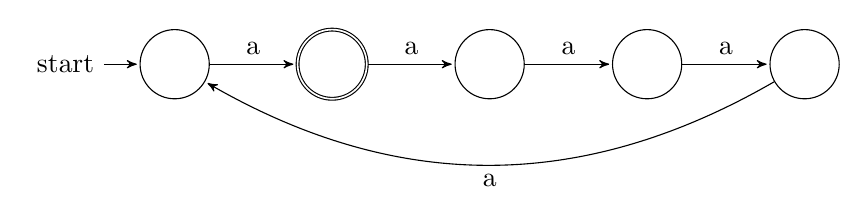
\begin{tikzpicture}[>=stealth',shorten >=1pt,auto,node distance=2cm]
    \node[initial,state] (1) {};
    \node[state, accepting] (2) [right of=1]{};
    \node[state] (3) [right of=2]{};
    \node[state] (4) [right of=3]{};
    \node[state] (5) [right of=4]{};

    \path[->] (1) edge node {a} (2);
    \path[->] (2) edge node {a} (3);
    \path[->] (3) edge node {a} (4);
    \path[->] (4) edge node {a} (5);
    \path[->] (5) edge [bend left] node {a} (1);
\end{tikzpicture}

A single {\tt a} or a sequence of {\tt a}'s increasing by 5 each time.

\part[5] 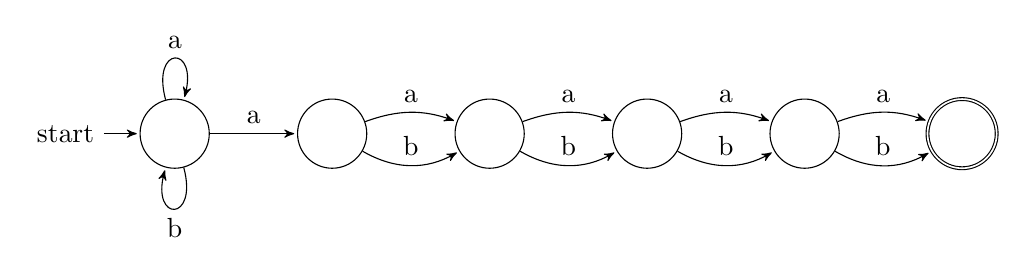
\begin{tikzpicture}[>=stealth',shorten >=1pt,auto,node distance=2cm]
    \node[initial,state] (1) {};
    \node[state] (2) [right of=1]{};
    \node[state] (3) [right of=2]{};
    \node[state] (4) [right of=3]{};
    \node[state] (5) [right of=4]{};
    \node[state, accepting] (6) [right of=5]{};

    \path[->] (1) edge node {a} (2);
    \path[->] (2) edge [bend right=-20] node {a} (3);
    \path[->] (2) edge [bend right] node {b} (3);
    \path[->] (3) edge [bend right=-20] node {a} (4);
    \path[->] (3) edge [bend right] node {b} (4);
    \path[->] (4) edge [bend right=-20] node {a} (5);
    \path[->] (4) edge [bend right] node {b} (5);
    \path[->] (5) edge [bend right=-20] node {a} (6);
    \path[->] (5) edge [bend right] node {b} (6);
    \path[->] (1) edge [loop above] node {a} (1);
    \path[->] (1) edge [loop below] node {b} (1);
\end{tikzpicture}

Any number of {\tt a}'s or {\tt b}'s, followed by an {\tt a}, followed by a comibination of 4 {\tt a}'s and {\tt b}'s.

\end{parts}

\question[6]
Write a regular expression whose language is equivalent to the following NFA.

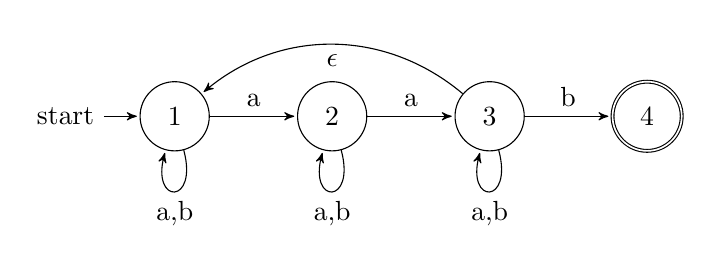
\begin{tikzpicture}[>=stealth',shorten >=1pt,auto,node distance=2cm]
    \node[initial,state] (1) {1};
    \node[state] (2) [right of=1]{2};
    \node[state] (3) [right of=2]{3};
    \node[state, accepting] (4) [right of=3]{4};

    \path[->] (1) edge node {a} (2);
    \path[->] (2) edge node {a} (3);
    \path[->] (3) edge node {b} (4);
    \path[->] (3) edge [bend left=-40] node {$\epsilon$} (1);
    \path[->] (1) edge [loop below] node {a,b} (1);
    \path[->] (2) edge [loop below] node {a,b} (2);
    \path[->] (3) edge [loop below] node {a,b} (3);
\end{tikzpicture}

$((a|b)^{*}a(a|b)^{*}a(a|b)^{*})^{+}b$

\question
Convert these NFAs into DFAs.

\begin{parts}
\part[6]
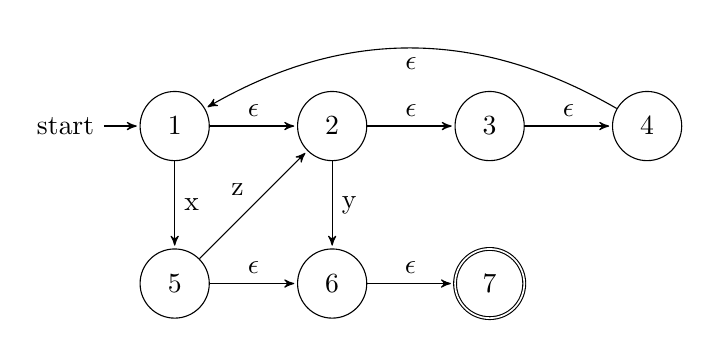
\begin{tikzpicture}[>=stealth',shorten >=1pt,auto,node distance=2cm]
    \node[initial,state] (1) {1};
    \node[state] (2) [right of=1]{2};
    \node[state] (3) [right of=2]{3};
    \node[state] (4) [right of=3]{4};
    \node[state] (5) [below of=1]{5};
    \node[state] (6) [right of=5]{6};
    \node[state, accepting] (7) [right of=6]{7};

    \path[->] (1) edge node {$\epsilon$} (2);
    \path[->] (2) edge node {$\epsilon$} (3);
    \path[->] (3) edge node {$\epsilon$} (4);
    \path[->] (1) edge node {x} (5);
    \path[->] (5) edge node {$\epsilon$} (6);
    \path[->] (6) edge node {$\epsilon$} (7);
    \path[->] (2) edge node {y} (6);
    \path[->] (5) edge node {z} (2);
    \path[->] (4) edge [bend left=-30] node {$\epsilon$} (1);
\end{tikzpicture}

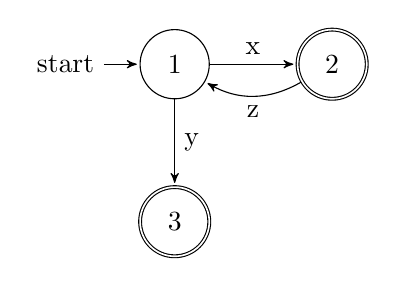
\begin{tikzpicture}[>=stealth',shorten >=1pt,auto,node distance=2cm]
    \node[state, initial] (1) {1};
    \node[state, accepting] (2) [right of=1] {2};
    \node[state, accepting] (3) [below of=1] {3};

    \path[->](1) edge node {x} (2);
    \path[->](1) edge node {y} (3);
    \path[->](2) edge [bend left=30] node {z} (1);
\end{tikzpicture}

\part[6]
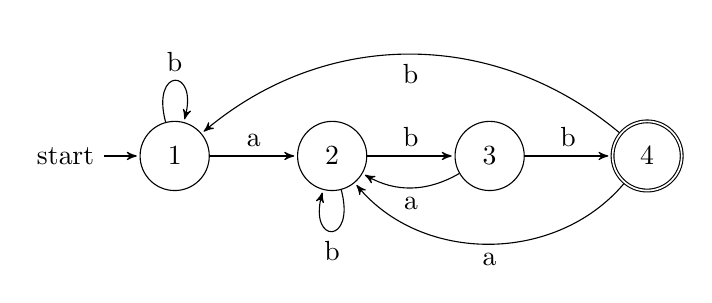
\begin{tikzpicture}[>=stealth',shorten >=1pt,auto,node distance=2cm]
    \node[initial,state] (1) {1};
    \node[state] (2) [right of=1]{2};
    \node[state] (3) [right of=2]{3};
    \node[state, accepting] (4) [right of=3]{4};

    \path[->] (1) edge [loop above] node {b} (1);
    \path[->] (1) edge node {a} (2);
    \path[->] (2) edge node {b} (3);
    \path[->] (3) edge node {b} (4);
    \path[->] (4) edge [bend left=-40] node {b} (1);
    \path[->] (4) edge [bend left=50] node {a} (2);
    \path[->] (3) edge [bend left] node {a} (2);
    \path[->] (2) edge [loop below] node {b} (2);
\end{tikzpicture}

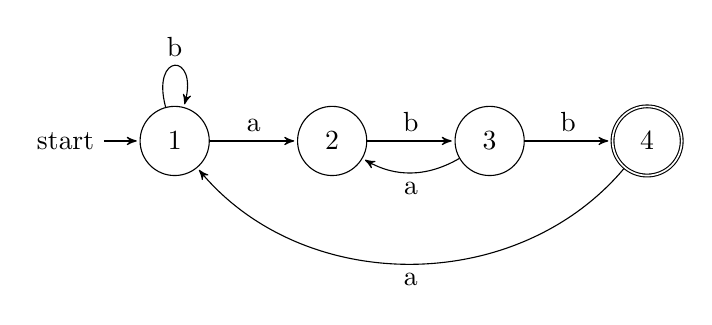
\begin{tikzpicture}[>=stealth',shorten >=1pt,auto,node distance=2cm]
    \node[state, initial] (1) {1};
    \node[state] (2) [right of=1] {2};
    \node[state] (3) [right of=2] {3};
    \node[state, accepting] (4) [right of=3] {4};

    \path[->] (1) edge [loop above] node {b} (1);
    \path[->] (1) edge node {a} (2);
    \path[->] (2) edge node {b} (3);
    \path[->] (3) edge node {b} (4);
    \path[->] (3) edge [bend left=30] node {a} (2);
    \path[->] (4) edge [bend left=50] node {a} (1);
\end{tikzpicture}

\end{parts}

\question
Construct DFA's for each of the following regular expressions. Do it in two steps: construct the NFA using Thompson's construction, then the DFA from the NFA. Let the alphabet be \{a,b\}.

\begin{parts}
\part[6] \begin{verbatim}a*|b*\end{verbatim}

\begin{figure}[H]
\centering
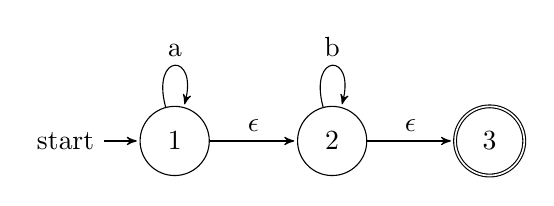
\begin{tikzpicture}[>=stealth',shorten >=1pt,auto,node distance=2cm]
    \node[state, initial] (1) {1};
    \node[state] (2) [right of=1] {2};
    \node[state, accepting] (3) [right of=2] {3};

    \path[->] (1) edge [loop above] node {a} (1);
    \path[->] (1) edge node {$\epsilon$} (2);
    \path[->] (2) edge [loop above] node {b} (2);
    \path[->] (2) edge node {$\epsilon$} (3);
\end{tikzpicture}
\caption{NFA}
\end{figure}

\begin{figure}[H]
\centering
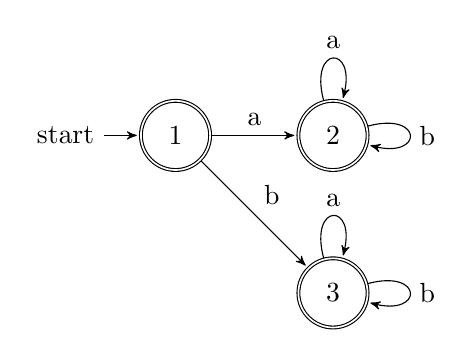
\begin{tikzpicture}[>=stealth',shorten >=1pt,auto,node distance=2cm]
    \node[state, initial, accepting] (1) {1};
    \node[state, accepting] (2) [right of=1] {2};
    \node[state, accepting] (3) [below of=2] {3};

    \path[->] (1) edge node {a} (2);
    \path[->] (1) edge node {b} (3);
    \path[->] (2) edge [loop above] node {a} (2);
    \path[->] (2) edge [loop right] node {b} (2);
    \path[->] (3) edge [loop above] node {a} (3);
    \path[->] (3) edge [loop right] node {b} (3);
\end{tikzpicture}
\caption{DFA}
\end{figure}

\part[7] \begin{verbatim}a*(ab)*a*\end{verbatim}

\begin{figure}[H]
\centering
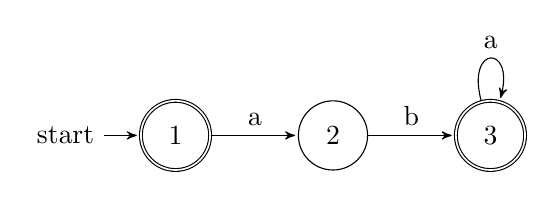
\begin{tikzpicture}[>=stealth',shorten >=1pt,auto,node distance=2cm]
    \node[state, initial, accepting] (1) {1};
    \node[state] (2) [right of=1] {2};
    \node[state, accepting] (3) [right of=2] {3};

    \path[->] (1) edge node {a} (2);
    \path[->] (2) edge node {b} (3);
    \path[->] (3) edge [loop above] node {a} (3);
\end{tikzpicture}
\caption{NFA}
\end{figure}

\begin{figure}[H]
\centering
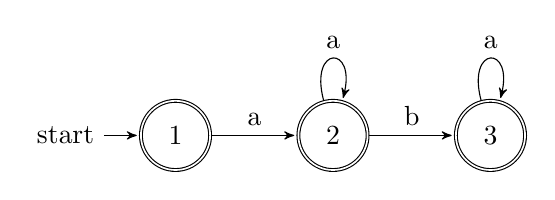
\begin{tikzpicture}[>=stealth',shorten >=1pt,auto,node distance=2cm]
    \node[state, initial, accepting] (1) {1};
    \node[state, accepting] (2) [right of=1] {2};
    \node[state, accepting] (3) [right of=2] {3};

    \path[->] (1) edge node {a} (2);
    \path[->] (2) edge [loop above] node {a} (2);
    \path[->] (2) edge node {b} (3);
    \path[->] (3) edge [loop above] node {a} (3);
\end{tikzpicture}
\caption{DFA}
\end{figure}

\part[7] {\bf CSC416 ONLY: } \begin{verbatim}[ab]*abab\end{verbatim}

\begin{figure}[H]
\centering
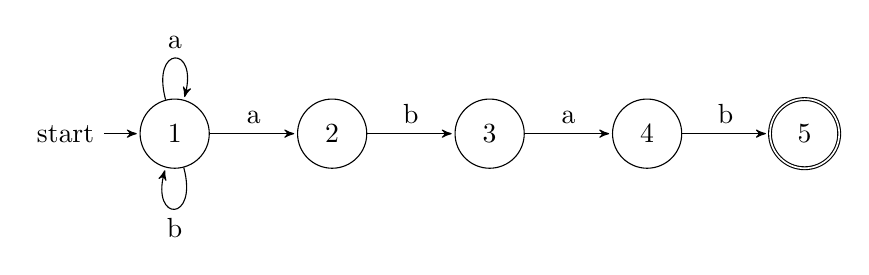
\begin{tikzpicture}[>=stealth',shorten >=1pt,auto,node distance=2cm]
    \node[state, initial] (1) {1};
    \node[state] (2) [right of=1] {2};
    \node[state] (3) [right of=2] {3};
    \node[state] (4) [right of=3] {4};
    \node[state, accepting] (5) [right of=4] {5};

    \path[->] (1) edge node {a} (2);
    \path[->] (1) edge [loop above] node {a} (1);
    \path[->] (1) edge [loop below] node {b} (1);
    \path[->] (2) edge node {b} (3);
    \path[->] (3) edge node {a} (4);
    \path[->] (4) edge node {b} (5);
\end{tikzpicture}
\caption{NFA}
\end{figure}

\begin{figure}[H]
\centering
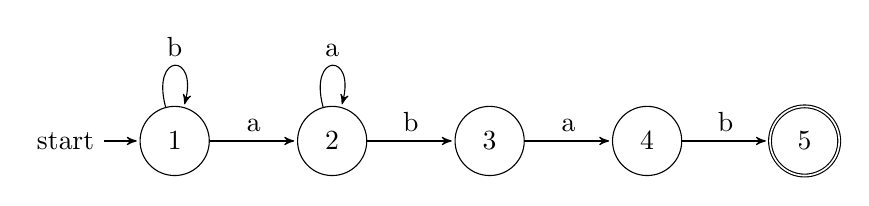
\begin{tikzpicture}[>=stealth',shorten >=1pt,auto,node distance=2cm]
    \node[state, initial] (1) {1};
    \node[state] (2) [right of=1] {2};
    \node[state] (3) [right of=2] {3};
    \node[state] (4) [right of=3] {4};
    \node[state, accepting] (5) [right of=4] {5};

    \path[->] (1) edge node {a} (2);
    \path[->] (1) edge [loop above] node {b} (1);
    \path[->] (2) edge node {b} (3);
    \path[->] (2) edge [loop above] node {a} (2);
    \path[->] (3) edge node {a} (4);
    \path[->] (4) edge node {b} (5);
\end{tikzpicture}
\caption{DFA}
\end{figure}

{\bf CSC565 ONLY: } \begin{verbatim}[ab]*abab[ab]*\end{verbatim}

\begin{figure}[H]
\centering
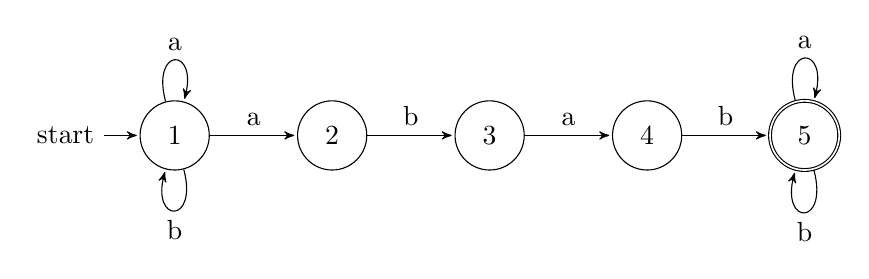
\begin{tikzpicture}[>=stealth',shorten >=1pt,auto,node distance=2cm]
    \node[state, initial] (1) {1};
    \node[state] (2) [right of=1] {2};
    \node[state] (3) [right of=2] {3};
    \node[state] (4) [right of=3] {4};
    \node[state, accepting] (5) [right of=4] {5};

    \path[->] (1) edge node {a} (2);
    \path[->] (1) edge [loop above] node {a} (1);
    \path[->] (1) edge [loop below] node {b} (1);
    \path[->] (2) edge node {b} (3);
    \path[->] (3) edge node {a} (4);
    \path[->] (4) edge node {b} (5);
    \path[->] (5) edge [loop above] node {a} (5);
    \path[->] (5) edge [loop below] node {b} (5);
\end{tikzpicture}
\caption{NFA}
\end{figure}

\begin{figure}[H]
\centering
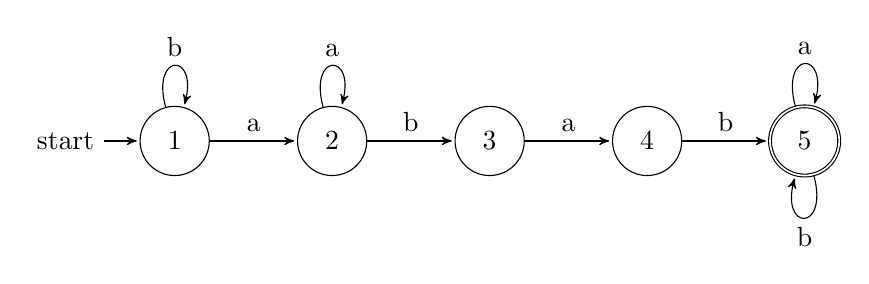
\begin{tikzpicture}[>=stealth',shorten >=1pt,auto,node distance=2cm]
    \node[state, initial] (1) {1};
    \node[state] (2) [right of=1] {2};
    \node[state] (3) [right of=2] {3};
    \node[state] (4) [right of=3] {4};
    \node[state, accepting] (5) [right of=4] {5};

    \path[->] (1) edge node {a} (2);
    \path[->] (1) edge [loop above] node {b} (1);
    \path[->] (2) edge node {b} (3);
    \path[->] (2) edge [loop above] node {a} (2);
    \path[->] (3) edge node {a} (4);
    \path[->] (4) edge node {b} (5);
    \path[->] (5) edge [loop above] node {a} (5);
    \path[->] (5) edge [loop below] node {b} (5);
\end{tikzpicture}
\caption{DFA}
\end{figure}

\end{parts}

\end{questions}

\end{document}
